%!TEX TS-program = pdflatex

\documentclass[10pt,a4paper,italian]{article} %classe book, A4 con pt 10

\usepackage[utf8]{inputenc} %codifica il documento con UTF8
\usepackage[italian]{babel}
\usepackage{amsmath} %Arricchisce la scelta nel comporre le formule.
\usepackage{amssymb} %idem
\usepackage{graphicx} %facilita la gestione delle figure
\usepackage{amsfonts}

\graphicspath{ {images/} } %le immagini sono nella cartella images
\pagestyle{plain} %lascia vuota la testata e mette il numero di pagina centrato nel piede

\author{Stefano Orioli}
\title{Sistemi flessibili per la cattura di traffico bluetooth}
\date{14/02/2018}




\begin{document}

\maketitle %stampo il titolo


\tableofcontents %stampo l'indice


%!TEX root = Tesi.tex

\section{Bluetooth Low Energy}
\subsection{Introduzione}
Il Bluetooth Low Energy (BLE) è una tecnologia wireless introdotta nello standard 4.0, disegnata e commercializzata dal SIG\footnote{Bluetooth Special Interest Group: organizzazione che regolamenta e definisce gli standard  per la trasmissione dati tramite la tecnologia Bluetooth.}; ideata per trasmissioni di dati di breve dimensione, essa si differenzia dal Bluetooth classico per un inferiore consumo di energia, mantenendo la stessa portata trasmissiva.

\subsection{Banda Trasmissiva}
BLE opera alla stessa banda di frequenza del bluetooth classico, 2,400 - 2,4835 GHz, ma utilizza un numero inferiore di canali, 40 canali da 2 MHz l'uno.
Nel canale trasmissivo i dati sono trasmessi con una modulazione GFSK.\footnote{Gaussin Frequency Shift Keying, limita la larghezza dello spettro trasmissivo tramite un filtro di tipo Gaussiano.}
I bitrate trasmissivi sono limitati ai valori 125 kbit/s, 1 Mbit/s o 2 Mbit/s.

Bluetooth Low Energy utilizza il \emph{Frequency Hopping}, una tecnica trasmissiva che consiste nel cambiare canale trasmissivo per ogni pacchetto inviato durante una trasmissione; l'utilizzo di questa tecnica permette di ridurre i problemi di interferenza con gli altri canali ed allo stesso tempo di aumentare la sicurezza delle trasmissioni.

\subsection{Stack protocollare}
Storicamente lo stack Bluetooth è diviso in 2 componenti fondamentali: il \emph{Controller} e l'\emph{Host}.
La parte di Controller è quella che si occupa di eseguire le componenti di basso livello dello stack necessarie per gestire i pacchetti scambiati a livello fisico e le loro temporizzazioni; la parte di Host comprende le componenti di alto livello tra cui profili e API\footnote{Application Program Interface: insieme di procedure utili a svolgere uno specifico compito}. La parte di Host, diversamente da quella di controllo, astrae dall'hardware ed è caratterizzata da una gestione meno rigida delle temporizzazioni.

L'\emph{HCI}\footnote{Host Controller Interface}, l'interfaccia tra Host e Controller si occupa di mettere in comunicazione queste due componenti fondamentali, utilizzando canali comunicativi quali UART o USB.
Se i due componenti sono montati su uno stesso chip, come nel caso dei SoC\footnote{System on a Chip: sistema completamente contenuto su un solo Chip}, allora l'interfaccia HCI è opzionale e può essere omessa.

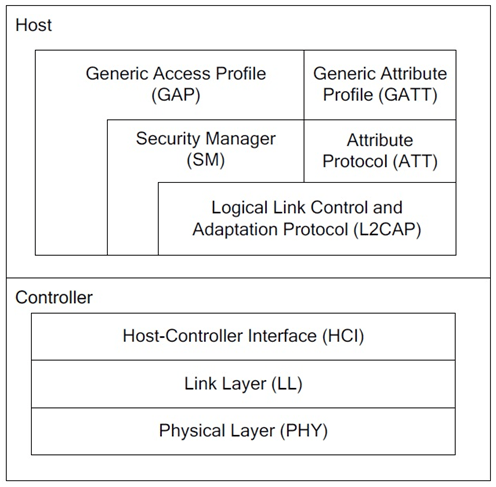
\includegraphics[scale=0.5]{stack_ble.png}

\begin{itemize}
\item Physical Layer (PHY): è il livello fisico, ovvero l'etere; lavora nella banda di frequenza 2,4 GHz ISM\footnote{Industrial, Scientific and Medical: frequenze riservate alle applicazioni di radiocomunicazioni non commerciali, ovvero per uso industriale, scientifico e medico.} Si compone di 40 canali da 2 MHz ognuno suddivisi in 3 per advertising e 37 per lo scambio dati.

\item Link Layer (LL): si occupa della gestione della sequenza e della temporizzazione dei pacchetti scambiati. Dialoga con i nodi vicini e scambia informazioni quali i parametri di connessione e controllo di flusso.\linebreak 
\'E una macchina a stati che si compone di 5 stati: Standby, Advertising, Scanning, Initiating, Connection. 

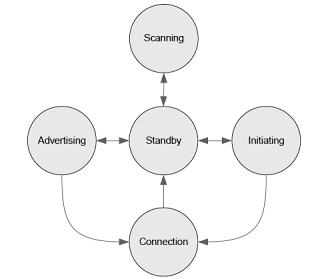
\includegraphics[scale=0.5]{LL_states}

\begin{itemize}

\item Advertising: il dispositivo rende noto agli ascoltatori della propria presenza, indicando la disponibilità ad una connessione ed inviando alcune informazioni utili.

\item Scanning: il dispositivo è in ascolto di tutte le informazioni trasmesse sui canali di advertise.

\item Initiating: un dispositivo in ascolto individua un Advertise di suo interesse ed indica la sua volontà di connettersi.

\item Connection: due o più dispositivi sono connessi.

\item Standby: il dispositivo è in uno stato di attesa caratterizzato da un basso consumo energetico.

\end{itemize}

Lo stato di Scanning può essere attivo (richiede informazioni aggiuntive) o passivo; Lo stato Connection anch'esso si divide in 2 sottostati: Central e Peripheral.

\item Logical Link Control and Adaptation Protocol (L2CAP): fornisce servizi sui dati ai livelli superiori, come ad esempio il Security Manager Protocol o l'Attribute Protocol. \'E responsabile inoltre della segmentazione e ricostruzione dei pacchetti da e verso i livelli inferiori.

\item Security Manager (SM): è responsabile del pairing dei dispositivi e della distribuzione delle chiavi crittografiche; BLE utilizza lo standard AES-128 bit per la cifratura dei dati ed il sistema di pairing per la distribuzione delle chiavi.

\item Attribute Protocol (ATT): gestisce la distribuzione delle informazioni riguardanti le coppie attributo-valore presenti in un device peripheral (Server)

\item Generic Access Profile (GAP): controlla \emph{advertising} e \emph{connection} . Divide i dispositivi bluetooth low energy in:
\begin{itemize}
\item Peripheral: normalmente dispositivi dotati di una limitata capacità di calcolo, come ad esempio un sensore di temperatura.
\item Central: dispositivo che gestisce la rete bluetooth e che richiede una maggiore capacità di calcolo; mentre un dispositivo periferico può avere una connessione con un solo dispositivo centrale, un centrale può gestire più dispositivi periferici andando a creare una Piconet\footnote{Rete Bluetooth composta da massimo otto dispositivi in relazione master-slave e fino a 255 dispositivi in modalità inattiva o parcheggio.}
\end{itemize} 

\item Generic Attribute Profile (GATT): entra in gioco a connessione avvenuta, definisce il modo in cui 2 dispositivi BLE scambiano dati utilizzando i concetti di \emph{Services} e \emph{Characteristics}.

\begin{itemize}
\item GATT server: è un peripheral device, che tramite il protocollo ATT permette al central di conoscere i dati che ha memorizzato in strutture di tipo service-characteristic.
\item GATT client: è il central device, che gestisce le comunicazioni e che richiede ai server periferici i dati raccolti.
\end{itemize}



\end{itemize}



 


\end{document}\grid
\grid
